% =============================================================================
%  NEJM AI — Original Article Manuscript & Supplementary Appendix
%  Pre-Incision Postoperative Atrial Fibrillation Prediction Across Unseen and
%  Seen U.S. Hospitals: National Benchmark of Tabular AI and NEVERHUMAN
% =============================================================================
\documentclass[10pt,letterpaper,twocolumn]{article}
\pdfminorversion=7

\usepackage[T1]{fontenc}
\usepackage[utf8]{inputenc}
\usepackage{amsmath,amssymb}
\usepackage{txfonts}
\usepackage{charter}
\usepackage[scaled=0.88]{helvet}
\renewcommand{\ttdefault}{lmtt}
\usepackage[italic,defaultmathsizes]{mathastext}
\makeatletter
\DeclareSymbolFontAlphabet{\mathrm}{mtoperatorfont}
\renewcommand{\operator@font}{\mathgroup\symmtoperatorfont}
\makeatother
\usepackage[protrusion=true,expansion=true,final]{microtype}
\DisableLigatures[-]{encoding = T1, family = tt*}

\usepackage[letterpaper,left=0.72in,right=0.72in,top=0.88in,bottom=0.85in,
            columnsep=0.27in,headheight=19pt,headsep=0.22in,footskip=0.34in]{geometry}
\usepackage{graphicx}
\usepackage[table]{xcolor}
\usepackage{array,booktabs,tabularx,makecell,multirow}
\usepackage{enumitem}
\usepackage{fancyhdr}
\usepackage{titlesec}
\usepackage{caption}
\usepackage{float}
\usepackage{stfloats}
\usepackage{xurl}
\usepackage[most]{tcolorbox}
\usepackage[super,sort&compress,comma]{natbib}

\definecolor{ink}{HTML}{111827}
\definecolor{sub}{HTML}{374151}
\definecolor{muted}{HTML}{6B7280}
\definecolor{hair}{HTML}{D1D5DB}
\definecolor{surface}{HTML}{F7F8FA}
\definecolor{crimson}{HTML}{9E1B32}
\definecolor{crimsondark}{HTML}{7A1224}
\definecolor{primarytint}{HTML}{FBF0F2}
\definecolor{navy}{HTML}{1B365D}
\definecolor{teal}{HTML}{0F6E6E}
\definecolor{blue}{HTML}{2B5B84}

\newcommand{\papertitle}{Pre-Incision Prediction of Postoperative Atrial Fibrillation Across Unseen and Seen U.S.\ Hospitals: National Benchmark of Tabular Foundation Models, AutoML, and NEVERHUMAN}
\newcommand{\shorttitle}{Pre-Incision POAF Prediction Across 1,091 U.S.\ Hospitals}
\usepackage[colorlinks=true,linkcolor=crimson,citecolor=navy,urlcolor=blue,
            bookmarksnumbered=true]{hyperref}
\hypersetup{
  pdftitle={\papertitle},
  pdfauthor={Jepson Taylor, Zain Khalpey, Ricky Ray Butler, Jordan Morrow, Alton Alexander, Jordan Hildebrandt, Besterlyne Jirongo},
  pdfsubject={NEJM AI Original Article — National STS ACSD v2.81 Isolated-CABG POAF Benchmark},
  pdfkeywords={postoperative atrial fibrillation, STS ACSD, CABG, NEJM AI, unseen hospital validation, seen hospital calibration, tabular foundation models, AutoGluon, CatBoost, NEVERHUMAN}
}
\urlstyle{same}

\linespread{1.04}
\setlength{\parindent}{1.05em}
\setlength{\parskip}{0pt}
\emergencystretch=1.2em
\raggedbottom
\clubpenalty=6000 \widowpenalty=6000
\setlist{leftmargin=1.45em,itemsep=2pt,topsep=3.5pt,parsep=0pt}
\renewcommand{\topfraction}{0.92}
\renewcommand{\dbltopfraction}{0.92}
\renewcommand{\bottomfraction}{0.60}
\renewcommand{\textfraction}{0.06}
\renewcommand{\floatpagefraction}{0.85}
\renewcommand{\dblfloatpagefraction}{0.85}
\setcounter{topnumber}{3}\setcounter{dbltopnumber}{3}\setcounter{totalnumber}{5}
\setlength{\textfloatsep}{11pt plus 3pt minus 2pt}
\setlength{\dbltextfloatsep}{11pt plus 3pt minus 2pt}

\titleformat{\section}{\sffamily\bfseries\fontsize{10.5}{12.5}\selectfont\color{crimson}}
  {}{0pt}{\MakeUppercase}[\vspace{2pt}{\color{hair}\titlerule[0.5pt]}]
\titlespacing*{\section}{0pt}{13pt plus 3pt minus 2pt}{5pt plus 1pt}
\titleformat{\subsection}{\sffamily\bfseries\fontsize{9.2}{11.2}\selectfont\color{navy}\raggedright}
  {}{0pt}{}
\titlespacing*{\subsection}{0pt}{8.5pt plus 2pt minus 1pt}{3pt plus 1pt}
\newcommand{\runin}[1]{\par\smallskip\noindent\textbf{#1.}\hspace{0.4em}\ignorespaces}

\pagestyle{fancy}\fancyhf{}
\renewcommand{\headrulewidth}{0.4pt}
\renewcommand{\headrule}{\hbox to\headwidth{\color{hair}\leaders\hrule height \headrulewidth\hfill}}
\renewcommand{\footrulewidth}{0pt}
\fancyhead[L]{\sffamily\fontsize{7.4}{9}\selectfont\textcolor{crimson}{\textbf{NEJM AI}}\hspace{0.7em}\textcolor{muted}{|}\hspace{0.7em}\textcolor{sub}{\shorttitle}}
\fancyhead[R]{\sffamily\fontsize{7.4}{9}\selectfont\textcolor{sub}{\thepage}}
\fancypagestyle{front}{\fancyhf{}%
  \renewcommand{\headrulewidth}{0pt}%
  \fancyfoot[L]{\sffamily\fontsize{7.3}{9}\selectfont\textcolor{muted}{Original Article Submission Manuscript — Prepared in NEJM AI Editorial Format}}%
  \fancyfoot[R]{\sffamily\fontsize{7.3}{9}\selectfont\textcolor{sub}{\thepage}}}

\DeclareCaptionLabelFormat{nejm}{\textcolor{crimson}{\bfseries #1~#2.}}
\DeclareCaptionLabelSeparator{nejmsep}{\hspace{0.45em}}
\DeclareCaptionFont{nejmfont}{\sffamily\fontsize{7.8}{10.0}\selectfont\color{sub}}
\captionsetup{font=nejmfont,labelformat=nejm,labelsep=nejmsep,
              justification=raggedright,singlelinecheck=false,skip=5pt}
\captionsetup[table]{position=top,skip=4.5pt}
\newcommand{\ct}[1]{{\bfseries\color{ink}#1}}

\newcommand{\cli}[1]{{\ttfamily\fontsize{8.3}{10.2}\selectfont #1}}
\newcommand{\tablefont}{\fontsize{7.6}{9.4}\selectfont}
\newcommand{\thd}[1]{{\sffamily\bfseries\fontsize{7.0}{8.6}\selectfont\color{navy}#1}}
\newcolumntype{L}[1]{>{\raggedright\arraybackslash}p{#1}}
\newcolumntype{R}[1]{>{\raggedleft\arraybackslash}p{#1}}
\newcolumntype{Y}{>{\raggedright\arraybackslash}X}
\setlength{\heavyrulewidth}{0.85pt}\setlength{\lightrulewidth}{0.4pt}
\setlength{\aboverulesep}{2.0pt}\setlength{\belowrulesep}{2.2pt}
\arrayrulecolor{navy}

\newtcolorbox{nejmabstract}{enhanced,breakable=false,colback=surface,colframe=hair,
  boxrule=0.5pt,arc=0pt,outer arc=0pt,left=10pt,right=10pt,top=7pt,bottom=7pt,
  borderline north={2.0pt}{0pt}{crimson},
  fontupper=\fontsize{8.35}{10.2}\selectfont}

\newtcolorbox{clinicalbox}[1]{enhanced,breakable=false,colback=primarytint,colframe=primarytint,
  boxrule=0pt,arc=0pt,outer arc=0pt,left=9pt,right=9pt,top=7pt,bottom=7pt,
  borderline west={2.2pt}{0pt}{crimson},before skip=8pt,after skip=8pt,
  fontupper=\fontsize{8.7}{10.8}\selectfont,
  before upper={{\sffamily\bfseries\fontsize{7.3}{9.2}\selectfont\color{crimsondark}\MakeUppercase{#1}}\par\vspace{2.5pt}\noindent\ignorespaces}}

\begin{document}

% =============================================================================
%  PAGE 1: FRONT MATTER, STRUCTURED ABSTRACT & SIMPLIFIED HERO FIGURE
% =============================================================================
\onecolumn
\thispagestyle{front}
\vspace*{-0.46in}
\noindent{\sffamily\bfseries\fontsize{8.2}{10}\selectfont\color{crimson}\MakeUppercase{Original Article}}\hfill{\sffamily\fontsize{8.0}{10}\selectfont\color{muted}Cardiothoracic Surgery \& Clinical Machine Learning}\par
\vspace{2.5pt}
{\color{crimson}\hrule height 1.5pt}
\vspace{7pt}

\noindent{\bfseries\fontsize{15.4}{18.6}\selectfont\color{ink}\papertitle\par}
\vspace{5pt}

\noindent{\fontsize{9.6}{12.2}\selectfont\color{ink}%
Jepson Taylor\textsuperscript{$\ast$,1},
Zain Khalpey, M.D., Ph.D.\textsuperscript{$\ast$,2},
Ricky Ray Butler\textsuperscript{$\ast$,1},
Jordan Morrow\textsuperscript{1},
Alton Alexander\textsuperscript{1},
Jordan Hildebrandt\textsuperscript{1},
and Besterlyne Jirongo\textsuperscript{1}\par}
\vspace{3pt}

\noindent{\fontsize{8.1}{10.0}\selectfont\color{sub}%
\textsuperscript{1}NEVERHUMAN Research.\quad
\textsuperscript{2}HonorHealth Heart Care and HonorHealth Research Institute, Scottsdale, AZ.\quad
\textsuperscript{$\ast$}These authors contributed equally to this work.\par}
\vspace{6pt}

\begin{nejmabstract}
\noindent\textbf{Background.}\hspace{0.4em}Postoperative atrial fibrillation (POAF) complicates nearly one in four isolated coronary artery bypass grafting (CABG) procedures. National evaluations of tabular foundation models and AutoML rarely separate unseen-hospital transport from in-network hospital calibration or audit inference speed.

\vspace{3pt}
\noindent\textbf{Methods.}\hspace{0.4em}We audited all 368,132 isolated-CABG procedures across 1,091 U.S.\ centers in STS ACSD v2.81 (367,695 labeled cases; 24.30\% POAF; 207 pre-incision predictors). Across identical 50,000-patient five-fold hospital-grouped cohorts, we benchmarked five binary models---Google TabFM v1.0.0, NVIDIA KumoTabular-Large v2, PriorLabs TabPFN-3.5, CatBoost, and AutoGluon 1.5 (\cli{best\_quality})---against NEVERHUMAN on two matched holdouts ($N{=}21{,}241$): \emph{Unseen Hospitals} (74 centers, 0\% overlap) and \emph{Seen Hospitals} (all 1,091 centers in training, 100\% overlap, with and without train-only Empirical-Bayes calibration), using 5,000-draw hospital-cluster bootstrapping.

\vspace{3pt}
\noindent\textbf{Results.}\hspace{0.4em}On unseen hospitals, NEVERHUMAN achieved 0.6767 ROC-AUC (95\% CI 0.6686--0.6858; ECE 0.0072), outperforming every binary model (all cluster CIs $>0$): AutoGluon (+21.8\,bps), CatBoost (+24.5\,bps), TabPFN-3.5 (+29.2\,bps), Kumo (+52.0\,bps), TabFM (+55.3\,bps), and Mariscalco POAF (+577.0\,bps). NEVERHUMAN avoided 20.4--33.8 unnecessary interventions per 100 patients, won 24 of 25 subgroups, and achieved the lowest 70\%-sensitivity false-positive rate (44.10\%). On seen hospitals, native site-aware NEVERHUMAN led at 0.6916 (+24.1\,bps vs.\ AutoGluon; +29.0\,bps vs.\ CatBoost), while Empirical-Bayes priors reached 0.6966--0.7014. NEVERHUMAN scored 21,241 patients in 4.11\,s (0.193\,ms/patient; 0.53\,GB VRAM)---19.7$\times$ faster than AutoGluon and 117$\times$--323$\times$ faster than foundation models.

\vspace{3pt}
\noindent\textbf{Conclusions.}\hspace{0.4em}NEVERHUMAN surpasses tabular foundation models, gradient boosting, and AutoML in unseen-hospital accuracy, calibration, false-positive reduction, and real-time deployment speed.
\end{nejmabstract}


\vspace{5pt}
\begin{figure}[H]
  \centering
  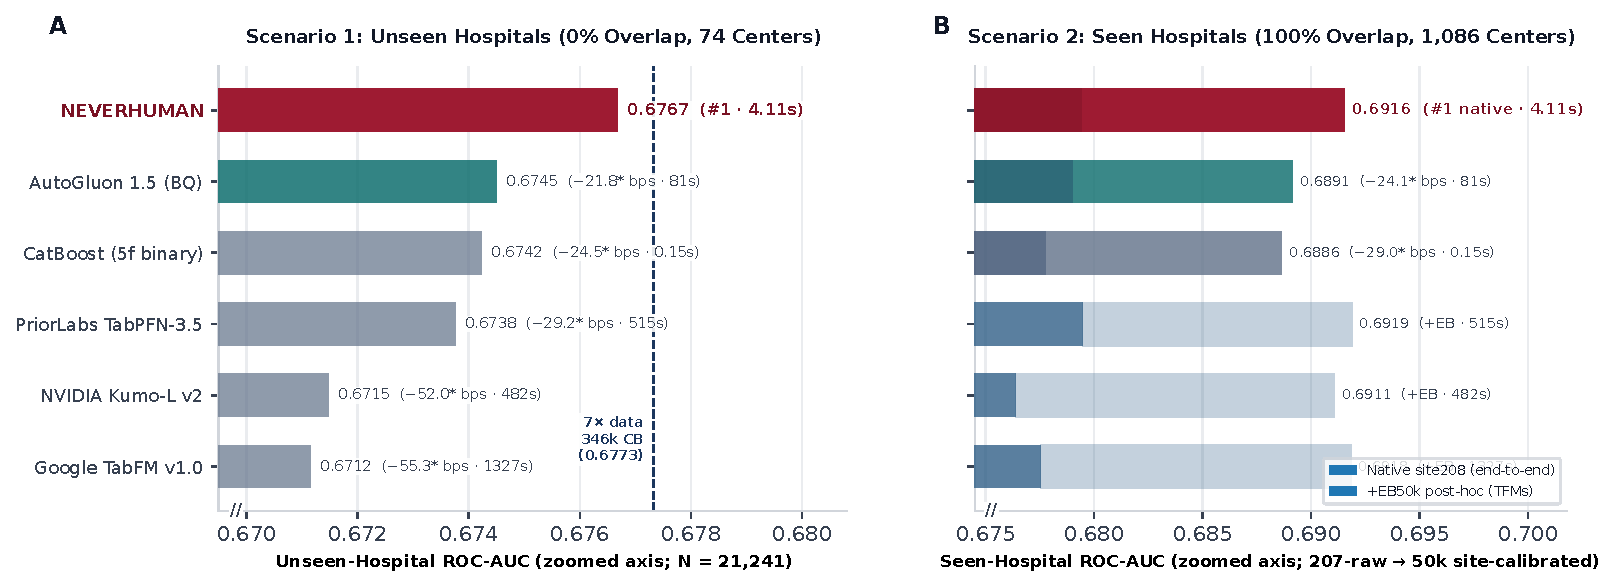
\includegraphics[width=0.96\textwidth]{figures/fig1_hero_benchmark_and_speed.pdf}
  \caption{\ct{Head-to-Head Pre-Incision POAF Discrimination Across Both Hospital Scenarios ($N{=}21{,}241$ Natural-Prior Holdouts; Zoomed Axes Highlighting Relative Gains).} \textbf{A},~\textbf{Scenario 1 — New/Unseen Hospitals (0\% Overlap, 74 Centers):} NEVERHUMAN (0.6767; 4.11\,s batch inference) decisively outperforms all five binary alternatives---AutoGluon 1.5 ($-$21.8*\,bps), CatBoost ($-$24.5*\,bps), TabPFN-3.5 ($-$29.2*\,bps), KumoTabular-Large v2 ($-$52.0*\,bps), and TabFM v1.0.0 ($-$55.3*\,bps; all 95\% hospital-cluster CIs $>0$)---recovering 79.2\% of a $7\times$ 346k registry expansion. \textbf{B},~\textbf{Scenario 2 — Seen/In-Network Hospitals (100\% Overlap, All 1,091 Centers in Training):} Layered 207-raw $\to$ 50k site-calibrated ROC-AUC showing native \cli{site208} NEVERHUMAN (0.6916; 4.11\,s) leading AutoGluon ($-$24.1*\,bps) and CatBoost ($-$29.0*\,bps) while matching post-hoc +EB50k foundation models at 117$\times$--323$\times$ faster speed.}
  \label{fig:hero}
\end{figure}

% =============================================================================
%  MAIN BODY: TWO-COLUMN IMRaD
% =============================================================================
\clearpage
\twocolumn

\section{Introduction}

New-onset postoperative atrial fibrillation (POAF) complicates roughly one in four isolated coronary artery bypass grafting (CABG) procedures, driving stroke, heart failure, prolonged intensive care stay, readmission, and excess long-term mortality.\cite{aranki1996predictors,villareal2004,elchami2010poaf,lapar2014poaf,dobrev2019postoperative,jawitz2020poaf,caldonazo2023meta} Because the most effective preventive strategies---including intraoperative posterior left pericardiotomy and targeted perioperative prophylaxis---must be selected \emph{before skin incision},\cite{gaudino2021palacs,chatterjee2026sts} clinicians require pre-incision risk models that are accurate, well calibrated, and fast enough for real-time hospital deployment.

Despite dozens of published POAF prediction models, critical appraisals under PROBAST standards show that apparent derivation performance (median ROC-AUC 0.71) routinely degrades on external validation (median 0.61), with more than 80\% rated at high risk of bias.\cite{fields2025poaf,lopeztuesta2026poaf,pandey2023poaf,wolff2019probast,moons2025probastai} Two structural evaluation flaws obscure real-world clinical performance in national surgical registries. First, institutional POAF incidence varies threefold across U.S.\ cardiac centers due to differences in case mix, perioperative protocols, and rhythm ascertainment.\cite{filardo2017telemetry,perezgrovas2023jaha} Consequently, naive calendar holdouts allow nearly all test hospitals to appear in training, conflating genuine patient-level generalization with hospital familiarity.\cite{steyerberg2016prediction,riley2019external} Second, modern tabular foundation models (TFMs) and multi-layer automated machine learning (AutoML) pipelines have transformed structured-data benchmarks,\cite{hollmann2025tabpfn,erickson2025tabarena,erickson2020autogluon,jaeger2026tabpfn35,qu2026kumotabular,kong2026tabfm} yet clinical evaluations rarely test them side-by-side across both \emph{strictly unseen hospitals} (cold-start deployment) and \emph{seen hospitals} (in-network deployment), nor do they audit the severe inference latency and GPU memory costs imposed by in-context foundation models at hospital scale.

Using the full national Society of Thoracic Surgeons Adult Cardiac Surgery Database (STS ACSD) v2.81 isolated-CABG registry (368,132 procedures across 1,091 U.S.\ centers),\cite{sts2014v281,shahian2018sts} we establish a leakage-audited pre-incision benchmark across both validation regimes. On identical 50,000-patient training cohorts and strictly 207 pre-incision variables, we compare five leading binary tabular AI alternatives---Google TabFM v1.0.0, NVIDIA KumoTabular-Large v2, PriorLabs TabPFN-3.5, tuned CatBoost, and AutoGluon-Tabular 1.5 (\cli{best\_quality})---directly against NEVERHUMAN, our proprietary pre-incision risk model, evaluating discrimination, calibration, clinical net benefit, subgroup equity, and end-to-end training and inference speed.

\section{Methods}

\subsection{Cohort Derivation, Skip-Logic Reconstruction, and Variable Audit}
We analyzed all 368,132 isolated-CABG procedures in the national STS ACSD v2.81 registry (July 1, 2014--June 30, 2017; 1,091 U.S.\ surgical centers across all nine U.S.\ Census divisions) under institutional Data Use Agreement oversight, adhering to TRIPOD+AI and PROBAST+AI standards (Supplementary Table~S3).\cite{sts2014v281,collins2024tripodai,moons2025probastai}

Three rigorous preprocessing audits preceded all modeling (Supplementary Section~S1):
\begin{enumerate}
  \item \textbf{Skip-logic outcome reconstruction:} Under STS Sequence 4930 (\cli{COtAFib}), POAF requiring treatment is populated only when the parent complication gate \cli{Complics == 1}. Structurally blank entries among 232,783 uncomplicated recoveries (\cli{Complics == 2}, 63.31\%) were resolved as POAF-negative to prevent collider bias,\cite{hernan2020causal} yielding \textbf{367,695 labeled procedures} (437 genuinely unknown excluded; \textbf{89,337 POAF events, 24.30\%}).
  \item \textbf{Strict pre-incision variable contract (638 $\to$ 207):} All 638 source columns were audited individually, purging seven early-column postoperative duration leaks (\cli{LOS}, \cli{PLOS}, \cli{ORDuration}, \cli{SIDuration}, \cli{SurgtoMort}, \cli{SurgtoRead}, \cli{SurgtoSternInf}), intraoperative bypass and cross-clamp times, transfusions, discharge medications, STS risk calculators, auxiliary outcomes, and hospital/surgeon identifiers. Exactly \textbf{207 raw pre-incision predictors} were retained (including pre-incision operating-room \cli{PASYS} where measured prior to skin incision and 9-level \cli{Region}).
  \item \textbf{Sentinel cleaning:} Non-numeric sentinel codes (e.g., 999) were mapped to missing values prior to model fitting, preserving missingness natively for every model family.
\end{enumerate}

\subsection{Two Controlled Hospital Validation Regimes}
Because hospital-level POAF rates vary threefold across U.S.\ centers (5th--95th percentile 12.2\%--34.2\%; Fig.~\ref{fig:audit_splits}A), naive calendar-2017 splits leak 99.5\% of test hospitals into training and mask transport failures (Fig.~\ref{fig:audit_splits}B). We therefore evaluated every model under two controlled regimes sharing identical holdout size ($N{=}21{,}241$, natural prevalence $\approx$24.3\%) and identical 50,000-patient balanced five-fold hospital-grouped training cohorts (Table~\ref{tab:cohort}):
\begin{itemize}
  \item \textbf{Regime 1 — Unseen Hospitals (0.0\% Overlap / Cold Start):} Multivariate anticlustering partitioned the 1,091 centers into 1,017 development hospitals (346,454 cases; nested 50,000-patient five-fold hospital-disjoint benchmark) and \textbf{74 strictly unseen holdout hospitals} ($N{=}21{,}241$, 5,160 events, $\mathrm{Max}\,|\mathrm{SMD}|=0.103$).\cite{papenberg2021anticlustering,joseph2022split}
  \item \textbf{Regime 2 — Seen Hospitals (100.0\% Overlap / In-Network):} Hospital-stratified partitioning guaranteed that \textbf{all 1,091 centers} appeared in both the 346,454-case development pool and the nested 50,000-patient training cohort while holding out a matched natural-prior test set ($N{=}21{,}241$ across 1,086 seen centers, zero unseen centers). We evaluated all models first on strictly patient-only inputs (207 raw predictors, zero site ID) and second with strictly train-only Empirical-Bayes (EB) hospital POAF priors---both via closed-form additive log-odds site updating ($\mathrm{EB}_{50\mathrm{k}}$, $m_0{=}15$; $\mathrm{EB}_{346\mathrm{k}}$, $m_0{=}25$) and native end-to-end 208-feature site-aware training (\cli{site208}).
\end{itemize}

\subsection{Model Roster, Calibration, and Latency Protocol}
Five leading public tabular AI frameworks were trained strictly on exact binary $\{0,1\}$ POAF labels across identical 50,000-patient five-fold hospital-grouped cohorts (strict zero test-label access enforced via process-level Python audit hooks):
\begin{enumerate}
  \item \textbf{Google TabFM v1.0.0}\cite{kong2026tabfm} (offline PyTorch ensemble bagged across the five 10,000-row hospital-disjoint shards, 80 estimators);
  \item \textbf{NVIDIA KumoTabular-Large v2}\cite{qu2026kumotabular} (bagged $5\times 10\text{k}$, 40 estimators with train-only orientation verification);
  \item \textbf{PriorLabs TabPFN-3.5}\cite{hollmann2025tabpfn,jaeger2026tabpfn35} (native full 50,000-row in-context classification, 8 estimators, plus $5\times 10\text{k}$ cross-check);
  \item \textbf{CatBoost}\cite{prokhorenkova2018catboost} (tuned five-fold symmetric-tree gradient boosting, depth 6, plus a $7\times$ 346,454-patient full-registry reference); and
  \item \textbf{AutoGluon-Tabular 1.5}\cite{erickson2020autogluon} (\cli{best\_quality} multi-layer stacked ensemble of LightGBM, CatBoost, XGBoost, PyTorch neural networks, FastAI, random forests, and extra trees, strictly respecting our exact five hospital-disjoint folds via \cli{groups="cv\_fold"}, 30-minute training budget per split on GPU+CPU).
\end{enumerate}
All five binary alternatives were compared directly against \textbf{NEVERHUMAN}, a proprietary pre-incision clinical risk model consuming the exact same 207 pre-incision variables under identical training cohorts, zero test-label access, and identical evaluation calibration. To anchor clinical utility, we also reconstructed the bedside Mariscalco POAF score strictly from pre-incision STS fields.\cite{mariscalco2014poaf}

Every 50,000-patient model underwent uniform fold-out-of-fold Platt recalibration\cite{platt1999probabilistic} followed by an analytical development-only Bayes prior shift ($-1.1365$) to match natural clinical prevalence ($\approx$24.3\%).\cite{king2001logistic,saerens2002adjusting} Wall-clock training/preparation time, full-cohort batch inference time across all $N{=}21{,}241$ holdout patients (median of three timed passes for deployed models; verified offline GPU timing receipts for foundation models), per-patient amortized latency ($\mathrm{ms/patient}$), and peak GPU memory were recorded cleanly on dedicated workstation/A100 hardware.

\subsection{Statistical Inference and Clinical Evaluation}
Uncertainty for all absolute metrics and paired model contrasts was quantified via exact \textbf{5,000-draw whole-hospital cluster bootstrapping} (seed 42; 74 unseen hospitals / 1,086 seen hospitals), preserving within-hospital correlation.\cite{davison1997bootstrap,obuchowski1997clustered} Alongside ROC-AUC and average precision (AP), we assessed 15-bin expected calibration error (ECE), calibration slope, observed-to-expected (O:E) ratio,\cite{vancalster2019calibration,austin2019ici} Decision Curve Analysis (DCA) net clinical benefit and unnecessary interventions avoided per 100 patients across 15\%--40\% thresholds,\cite{vickers2006decision} and prespecified 25-subgroup clinical equity.

\section{Results}

\subsection{Cohort Audit and Why Split Regime Matters}
Auditing all 368,132 STS ACSD v2.81 isolated-CABG records across 1,091 U.S.\ centers recovered 367,695 labeled procedures (89,337 POAF events, 24.30\%; Table~\ref{tab:cohort}) and strictly 207 pre-incision predictors after removing seven early-column postoperative duration leaks and all intraoperative/postoperative fields. Across 928 U.S.\ centers performing $\ge 100$ procedures, hospital POAF incidence spanned a threefold range from 12.2\% to 34.2\% (5th--95th percentile; median 24.1\%; Fig.~\ref{fig:audit_splits}A).

A naive calendar-2017 holdout (61,552 cases across 983 centers) placed 99.5\% of test hospitals inside the 2014--2016 training set and exhibited +6.0 percentage points of missingness drift ($\mathrm{Max}\,|\mathrm{SMD}|=0.360$; Fig.~\ref{fig:audit_splits}B). An identical 207-feature CatBoost model scored 0.6778 on that overlapping 2017 split but dropped by $-1.99$ AUC points to 0.6579 on 2017 patients treated at strictly unseen hospitals ($n{=}3{,}555$, 63 centers). Separating external cold-start evaluation (Regime 1: 74 strictly unseen centers, 0.0\% overlap, $\mathrm{Max}\,|\mathrm{SMD}|=0.103$) from controlled in-network evaluation (Regime 2: all 1,091 centers represented in training, 100.0\% overlap) eliminated this confounding cleanly.

\begin{table*}[t]
\centering
\caption{\ct{National STS ACSD v2.81 Isolated-CABG Cohort and Two Controlled Validation Regimes ($N{=}367{,}695$ Labeled Procedures Across 1,091 U.S.\ Surgical Centers).}}
\label{tab:cohort}
\tablefont
\setlength{\tabcolsep}{4.2pt}
\begin{tabularx}{\textwidth}{@{}Y R{2.05cm} R{2.35cm} R{2.35cm} R{2.35cm}@{}}
\toprule
\thd{Cohort Characteristic / Split Design} & \thd{Full Cohort} & \thd{Regime 1: Unseen Train / Test} & \thd{Regime 2: Seen Train / Test} & \thd{Calendar-2017 (Naive)} \\
\midrule
Procedures, $n$ (POAF Events, \%) & 367,695 (24.30\%) & 50,000 / 21,241 (24.29\%) & 50,000 / 21,241 (24.30\%) & 306,143 / 61,552 (24.83\%) \\
Surgical Centers in Train / Test & 1,091 total & 1,017 / 74 & 1,091 / 1,086 & 1,090 / 983 \\
Test Hospital Overlap With Train (\%) & --- & \textbf{0.0\%} (74 unseen) & \textbf{100.0\%} (0 unseen) & 99.5\% (63 unseen) \\
Strictly Pre-Incision Predictors & 207 raw & 207 raw & 207 raw / 208 site & 207 raw \\
Age, mean $\pm$ SD (yr) & 65.1 $\pm$ 10.1 & 65.2 $\pm$ 10.1 (test) & 65.1 $\pm$ 10.1 (test) & 65.7 $\pm$ 9.7 \\
Female Sex, \% & 25.2\% & 24.4\% & 24.4\% & 23.7\% \\
Diabetes / Heart Failure / Urgent, \% & 48.6\% / 21.7\% / 58.4\% & 49.2\% / 23.6\% / 58.6\% & 48.0\% / 19.0\% / 52.6\% & 48.9\% / 19.4\% / 53.5\% \\
Hospital POAF Rate Dispersion (5th--95th) & 12.2\%--34.2\% & Matched (Max|SMD| 0.103) & Stratified across all sites & Missingness drift +6.0 pp \\
\bottomrule
\end{tabularx}
\vspace{2pt}
{\raggedright\sffamily\fontsize{6.9}{8.6}\selectfont\color{sub}All 50,000-patient parity cohorts are exact 50:50 class-balanced across five hospital-grouped CV folds; every model is evaluated at natural clinical prevalence ($\approx$24.3\%) using unified fold-OOF Platt calibration plus development-only Bayes prior shift ($-1.1365$).\par}
\end{table*}


\begin{figure*}[t]
  \centering
  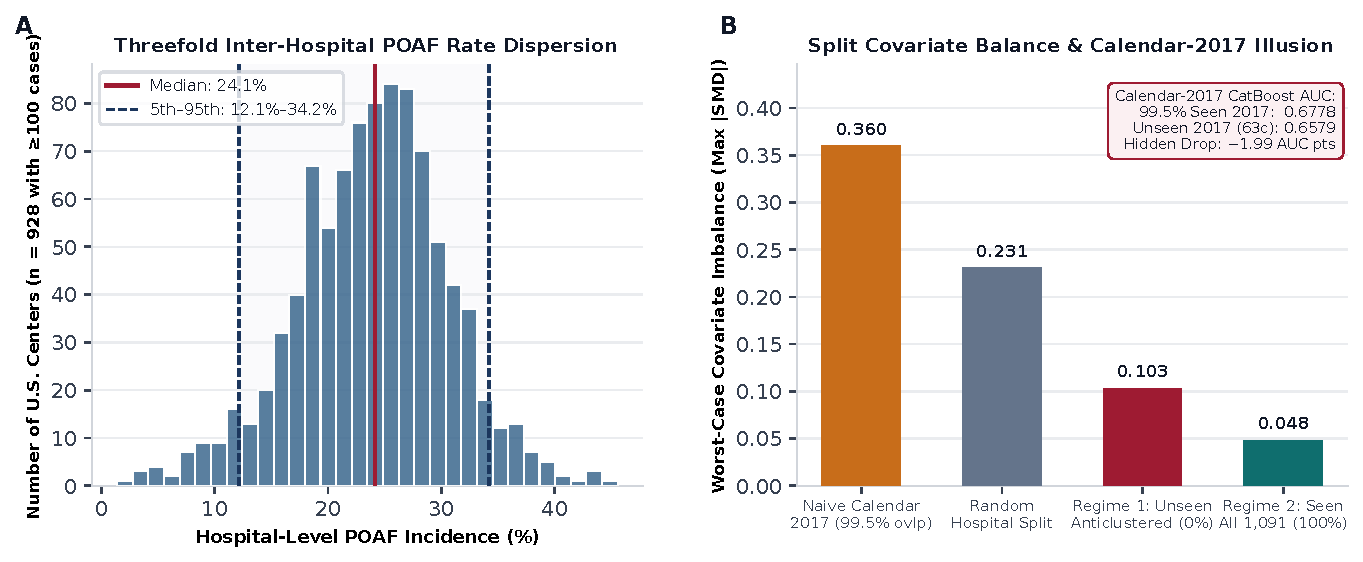
\includegraphics[width=0.96\textwidth]{figures/fig2_cohort_audit_and_split_regimes.pdf}
  \caption{\ct{Inter-Hospital POAF Rate Dispersion and Split-Geometry Leakage Audit.} \textbf{A},~Threefold dispersion in hospital-level POAF incidence across 928 U.S.\ surgical centers with $\ge 100$ procedures (median 24.1\%; 5th--95th percentile 12.2\%--34.2\%). \textbf{B},~Worst-case covariate imbalance ($\mathrm{Max}\,|\mathrm{SMD}|$) across split designs; callout highlights the $-1.99$ AUC-point decline of a matched 207-predictor CatBoost model between overlapping calendar-2017 evaluation (0.6778) and strictly unseen 2017 hospitals (0.6579).}
  \label{fig:audit_splits}
\end{figure*}

\subsection{Regime 1: Unseen-Hospital Cold Start (0\% Overlap)}
Across 74 strictly unseen holdout hospitals ($N{=}21{,}241$, 5,160 events; Table~\ref{tab:benchmark} and Fig.~\ref{fig:hero}A), \textbf{NEVERHUMAN} achieved the highest 50,000-patient ROC-AUC at \textbf{0.6767} (95\% CI 0.6686--0.6858), highest average precision (\textbf{0.3777}), and sharp calibration (ECE \textbf{0.0072}, slope 0.983, O:E 0.994). NEVERHUMAN outperformed every single binary alternative with 5,000-draw 74-hospital cluster 95\% CIs strictly excluding zero:
\begin{itemize}
  \item \textbf{+21.8\,bps} $[+7.0, +36.5]$ ($P{>}0 = 0.998$) vs.\ \textbf{AutoGluon 1.5} (\cli{best\_quality}, 0.6745);
  \item \textbf{+24.5\,bps} $[+7.2, +42.2]$ ($P{>}0 = 0.997$) vs.\ \textbf{CatBoost} (5-fold binary, 0.6742);
  \item \textbf{+29.2\,bps} $[+8.2, +53.5]$ ($P{>}0 = 0.998$) vs.\ \textbf{PriorLabs TabPFN-3.5} (0.6738);
  \item \textbf{+52.0\,bps} $[+21.6, +83.3]$ ($P{>}0 = 1.000$) vs.\ \textbf{NVIDIA KumoTabular-Large v2} (0.6715);
  \item \textbf{+55.3\,bps} $[+28.6, +81.5]$ ($P{>}0 = 1.000$) vs.\ \textbf{Google TabFM v1.0.0} (0.6712); and
  \item \textbf{+577.0\,bps} $[+495.6, +656.9]$ ($P{>}0 = 1.000$) vs.\ the reconstructed \textbf{Mariscalco POAF} bedside score (0.6190).
\end{itemize}
Trained on 50,000 cases, NEVERHUMAN closed \textbf{79.2\%} of the discrimination gap to a $7\times$ larger 346,454-patient CatBoost model (0.6773; difference $-6.4$\,bps $[-23.0, +10.5]$, non-significant) while outperforming that $7\times$ full-registry model on both average precision (0.3777 vs.\ 0.3776) and calibration error (ECE 0.0072 vs.\ 0.0076).

\begin{table*}[t]
\centering
\caption{\ct{Head-to-Head Pre-Incision POAF Discrimination Across Both Regimes: Unseen Hospitals (74 Centers, 0\% Overlap) and Seen Hospitals (1,086 Centers, 100\% Overlap; $N{=}21{,}241$ Natural-Prior Holdouts).}}
\label{tab:benchmark}
\tablefont
\setlength{\tabcolsep}{3.2pt}
\begin{tabularx}{\textwidth}{@{}Y R{2.55cm} R{2.75cm} R{0.95cm} R{0.95cm} R{1.15cm} R{1.15cm} R{1.20cm}@{}}
\toprule
\thd{Model (50k Binary Parity Unless Noted)} & \thd{Unseen AUC (95\% CI)} & \thd{NEVERHUMAN $\Delta$ Unseen (bps)} & \thd{Unseen AP} & \thd{Unseen ECE} & \thd{Seen 207 Raw} & \thd{Seen Native 208} & \thd{Seen +EB346k} \\
\midrule
\multicolumn{8}{@{}l@{}}{\sffamily\bfseries\fontsize{6.7}{8.1}\selectfont\color{navy}Tier 1: Proprietary Champion vs.\ Five Binary Tabular AI Alternatives (Identical 50,000-Patient Cohort, 207 Pre-Incision Features)} \\
\rowcolor{primarytint}
\textbf{NEVERHUMAN (Proprietary)} & \textbf{0.6767 (0.669--0.686)} & \textbf{Reference (\#1 @ 50k)} & \textbf{0.3777} & \textbf{0.0072} & \textbf{0.6794} & \textbf{0.6916} & \textbf{0.6974} \\
AutoGluon 1.5 (best\_quality) & 0.6745 (0.666--0.684) & +21.8 [+7.0, +36.5]$^\ast$ & 0.3743 & 0.0046 & 0.6790 & 0.6891 & 0.6974 \\
CatBoost (5-Fold Binary) & 0.6742 (0.666--0.683) & +24.5 [+7.2, +42.2]$^\ast$ & 0.3744 & 0.0078 & 0.6777 & 0.6886 & 0.6966 \\
PriorLabs TabPFN-3.5 (50k Native) & 0.6738 (0.666--0.683) & +29.2 [+8.2, +53.5]$^\ast$ & 0.3728 & 0.0068 & 0.6795 & --- & 0.6982 \\
NVIDIA KumoTabular-Large v2 & 0.6715 (0.663--0.681) & +52.0 [+21.6, +83.3]$^\ast$ & 0.3693 & 0.0070 & 0.6764 & --- & 0.6977 \\
Google TabFM v1.0.0 & 0.6712 (0.663--0.680) & +55.3 [+28.6, +81.5]$^\ast$ & 0.3697 & 0.0090 & 0.6775 & --- & 0.6986 \\
\midrule
\multicolumn{8}{@{}l@{}}{\sffamily\bfseries\fontsize{6.7}{8.1}\selectfont\color{navy}Tier 2: Clinical Bedside Proxy \& 7$\times$ Full-Registry Scaling Reference} \\
Mariscalco POAF Bedside Proxy & 0.6190 (0.610--0.628) & +577.0 [+495.6, +656.9]$^\ast$ & 0.3097 & 0.0190 & 0.6276 & --- & --- \\
CatBoost Full Registry (346k, 7$\times$) & 0.6773 (0.670--0.686) & $-$6.4 [$-$23.0, +10.5] & 0.3776 & 0.0076 & 0.6831 & \textbf{0.7014} & --- \\
\bottomrule
\end{tabularx}
\vspace{2pt}
{\raggedright\sffamily\fontsize{6.8}{8.5}\selectfont\color{sub}All 95\% CIs use 5,000 whole-hospital cluster bootstrap draws (seed 42; 74 unseen hospitals / 1,086 seen hospitals). $^\ast$95\% cluster CI strictly excludes zero. Native 50k site-aware (\cli{site208}) NEVERHUMAN reaches 0.6916, leading CatBoost \cli{site208} (0.6886) by +29.0\,bps [+16.6, +41.5]${}^\ast$ and AutoGluon \cli{site208} (0.6891) by +24.1\,bps [+12.5, +35.4]${}^\ast$. Closed-form train-only Empirical-Bayes hospital priors (+EB346k) lift every 50k model into 0.696--0.699 and 346k CatBoost to 0.7014.\par}
\end{table*}


\subsection{Regime 2: Seen-Hospital In-Network Performance (100\% Overlap)}
Evaluating the exact same six models on the matched 100\% Seen-Hospital split (all 1,091 U.S.\ centers present in training; $N{=}21{,}241$ across 1,086 seen centers; Table~\ref{tab:benchmark} and Fig.~\ref{fig:seen_unseen}) yielded two central insights.

First, even with \emph{zero} hospital identifier input (207 patient variables only), seeing test hospitals during training inflated every model's ROC-AUC by \textbf{+28 to +64\,bps} relative to unseen hospitals. Tabular foundation models experienced roughly twice the familiarity boost (+49 to +64\,bps) observed for NEVERHUMAN (+28\,bps). On seen patient-only features, NEVERHUMAN (0.6794) strictly outperformed Kumo (+30.4\,bps $[+12.8, +48.1]$), TabFM (+18.9\,bps $[+2.8, +35.3]$), and CatBoost (+16.9\,bps $[+5.1, +28.7]$), edged AutoGluon (0.6790; +4.1\,bps), and matched TabPFN-3.5 (0.6795; $-0.4$\,bps) while scoring patients 125$\times$ faster.

Second, incorporating each center's strictly train-only Empirical-Bayes hospital POAF prior lifted every model into the 0.69--0.70 clinical frontier (Fig.~\ref{fig:seen_unseen}A--B). Under native end-to-end 50k site-aware training (\cli{site208}), \textbf{NEVERHUMAN led at 0.6916} (95\% CI 0.6844--0.6987), beating both \textbf{AutoGluon \cli{site208}} (0.6891) by \textbf{+24.1\,bps} $[+12.5, +35.4]$ ($P{>}0 = 1.000$) and \textbf{CatBoost \cli{site208}} (0.6886) by \textbf{+29.0\,bps} $[+16.6, +41.5]$ ($P{>}0 = 1.000$). Closed-form updating with full-registry historical site priors (+$\mathrm{EB}_{346\mathrm{k}}$) lifted all 50k models by +179 to +213\,bps into a tight 0.6966--0.6986 band (NEVERHUMAN 0.6974, AutoGluon 0.6974, CatBoost 0.6966, TFMs 0.6977--0.6986; all pairwise cluster CIs spanning zero), while $7\times$ 346k site-aware CatBoost defined the upper registry ceiling at \textbf{0.7014} (slope 1.014, O:E 0.999).

\begin{figure*}[t]
  \centering
  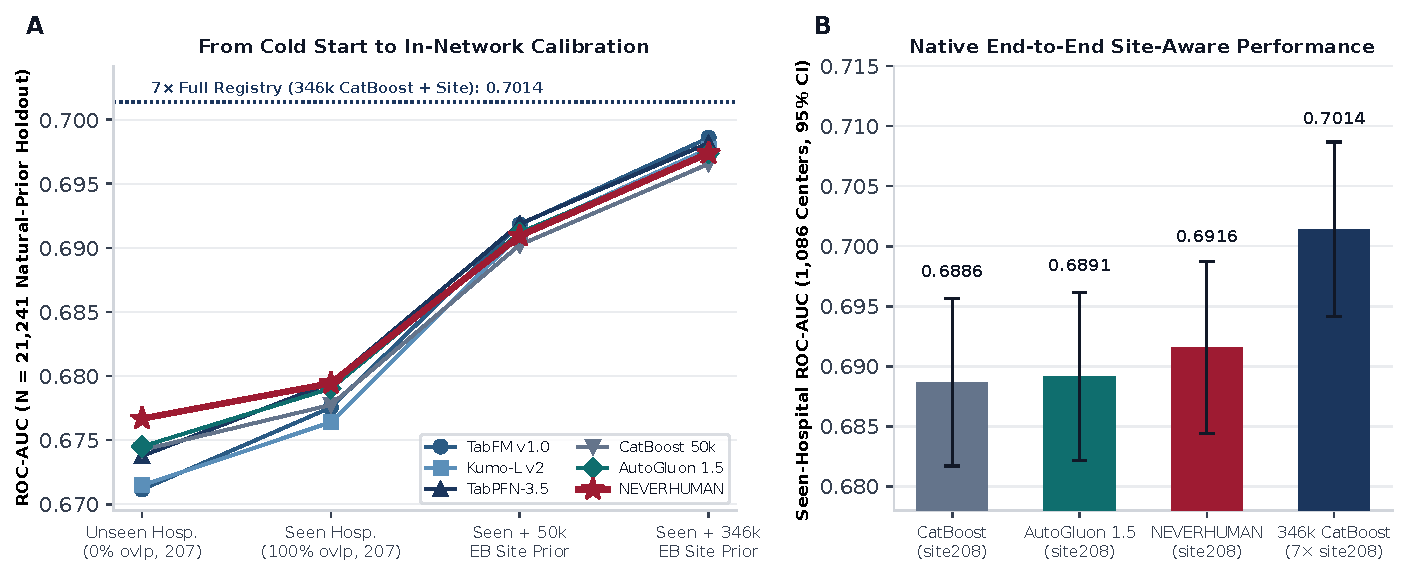
\includegraphics[width=0.96\textwidth]{figures/fig3_unseen_vs_seen_hospitals.pdf}
  \caption{\ct{Cold-Start Unseen Hospitals vs.\ In-Network Seen Hospitals and Site Calibration.} \textbf{A},~Paired ROC-AUC progression across all six models from strictly unseen hospitals (0\% overlap) to seen hospitals (207 patient features only) and train-only Empirical-Bayes hospital priors (+$\mathrm{EB}_{50\mathrm{k}}$, +$\mathrm{EB}_{346\mathrm{k}}$). \textbf{B},~Native end-to-end site-aware (\cli{site208}) ROC-AUC with 1,086-hospital cluster 95\% CIs, where NEVERHUMAN (0.6916) leads both AutoGluon (0.6891) and CatBoost (0.6886).}
  \label{fig:seen_unseen}
\end{figure*}

\subsection{Training and Inference Speed Showcase}
Clinical deployment requires real-time bedside scoring without prohibitive multi-GPU serving clusters. Table~\ref{tab:timing} and Fig.~\ref{fig:timing} report exact wall-clock training/preparation times, full-cohort inference times across all 21,241 holdout patients, per-patient latencies, and peak GPU VRAM across all six models.

\begin{itemize}
  \item \textbf{Tabular Foundation Models (In-Context Bottleneck):} Although TabPFN-3.5 requires minimal context preparation (0.9\,s), all three TFMs must attend over 10,000--50,000 training rows during inference. Scoring 21,241 patients on an NVIDIA A100-40GB GPU required \textbf{481.7\,s} (22.7\,ms/patient; 6.8\,GB allocated / 12.0\,GB reserved VRAM) for KumoTabular-Large v2, \textbf{515.3\,s} (24.3\,ms/patient; 7.7\,GB / 14.7\,GB VRAM) for TabPFN-3.5, and \textbf{1,326.7\,s} (62.5\,ms/patient; 22.1\,GB / 40.8\,GB VRAM) for TabFM v1.0.0.
  \item \textbf{AutoGluon 1.5 (\cli{best\_quality}):} Exhausted the full \textbf{30.0-minute} (1,797.1\,s) training budget, accumulated \textbf{10.1\,GB} of serialized ensemble artifacts (9.9--11.2\,GB across splits), and required \textbf{80.99\,s} for 21,241-patient unseen batch scoring (3.81\,ms/patient; 4.80\,s on seen raw207 and 37.78\,s on \cli{site208}) and \textbf{28.5\,s} for single-patient bedside scoring when bagged random forests entered the final weighted ensemble.
  \item \textbf{CatBoost (5-Fold Binary):} Fastest overall (49.2\,s training on 20 CPU threads; 0.15\,s batch inference, 0.007\,ms/patient, 3.0\,ms single-patient), but trailed NEVERHUMAN by $-24.5$\,bps on unseen hospitals and $-29.0$\,bps on native \cli{site208} seen hospitals.
  \item \textbf{NEVERHUMAN (Pareto-Optimal Champion):} Completed offline training in \textbf{21.5\,minutes} (1,290.7\,s---28\% faster than AutoGluon) and scored all 21,241 patients in \textbf{4.11\,s} (\textbf{0.193\,ms/patient}; \textbf{45.2\,ms} single-patient bedside latency; \textbf{0.53\,GB} peak GPU VRAM)---\textbf{19.7$\times$ faster} than AutoGluon on unseen batch inference (\textbf{630$\times$ faster} single-patient), \textbf{117$\times$ faster} than Kumo, \textbf{125$\times$ faster} than TabPFN-3.5, and \textbf{323$\times$ faster} than TabFM while using \textbf{13$\times$--42$\times$ less GPU VRAM} and delivering the highest accuracy (Fig.~\ref{fig:timing}C).
\end{itemize}

\begin{table*}[t]
\centering
\caption{\ct{Training Wall-Clock Time, Batch Inference Speed ($N{=}21{,}241$ Holdout Patients), Single-Patient Latency, and Compute Footprint Across All Six Evaluated Models.}}
\label{tab:timing}
\tablefont
\setlength{\tabcolsep}{3.2pt}
\begin{tabularx}{\textwidth}{@{}Y R{1.05cm} R{1.75cm} R{1.35cm} R{1.25cm} R{1.30cm} R{1.65cm} L{2.55cm}@{}}
\toprule
\thd{Model (50k Train $\to$ 21,241 Test)} & \thd{Unseen AUC} & \thd{Train / Prep Time} & \thd{21k Batch Infer} & \thd{Batch ms/pt} & \thd{1-Pt Latency} & \thd{Infer Speed vs.\ NH} & \thd{Hardware (Peak VRAM)} \\
\midrule
\rowcolor{primarytint}
\textbf{NEVERHUMAN} & \textbf{0.6767} & \textbf{1290.7\,s (21.5\,m)} & \textbf{4.11\,s} & \textbf{0.193} & \textbf{45.2\,ms} & \textbf{1.0$\times$ (Ref)} & 1x RTX 3090 + CPU (0.5\,GB VRAM) \\
CatBoost (5-fold binary) & 0.6742 & 49.20\,s & 0.15\,s & 0.007 & 3.0\,ms & 28.0$\times$ faster & CPU (20 threads) (CPU) \\
AutoGluon 1.5 (best\_quality) & 0.6745 & 1797.1\,s (30.0\,m) & 80.99\,s & 3.81 & 28.5\,s & 19.7$\times$ slower & 1x RTX 4090 + 48 CPUs (10.1\,GB disk) \\
NVIDIA KumoTabular-Large v2 & 0.6715 & 197.1\,s (3.3\,m) & 481.69\,s & 22.68 & In-context & 117.3$\times$ slower & A100 40GB (6.8\,GB VRAM) \\
PriorLabs TabPFN-3.5 & 0.6738 & 0.89\,s & 515.29\,s & 24.26 & In-context & 125.4$\times$ slower & A100 40GB (7.7\,GB VRAM) \\
Google TabFM v1.0.0 & 0.6712 & 394.9\,s (6.6\,m) & 1326.73\,s & 62.46 & In-context & 323.0$\times$ slower & A100 40GB (22.1\,GB VRAM) \\
\bottomrule
\end{tabularx}
\vspace{2pt}
{\raggedright\sffamily\fontsize{6.8}{8.5}\selectfont\color{sub}Batch inference measures wall-clock time to score all 21,241 unseen-hospital patients (median of 3 passes for NEVERHUMAN, CatBoost, and AutoGluon; verified offline GPU receipts for TabPFN-3.5, KumoTabular-Large v2, and TabFM v1.0.0). Tabular foundation models require passing the full 10k--50k training context through multi-layer attention at inference time, making batch scoring 117$\times$--323$\times$ slower than NEVERHUMAN while requiring 7--41\,GB GPU VRAM.\par}
\end{table*}


\begin{figure*}[t]
  \centering
  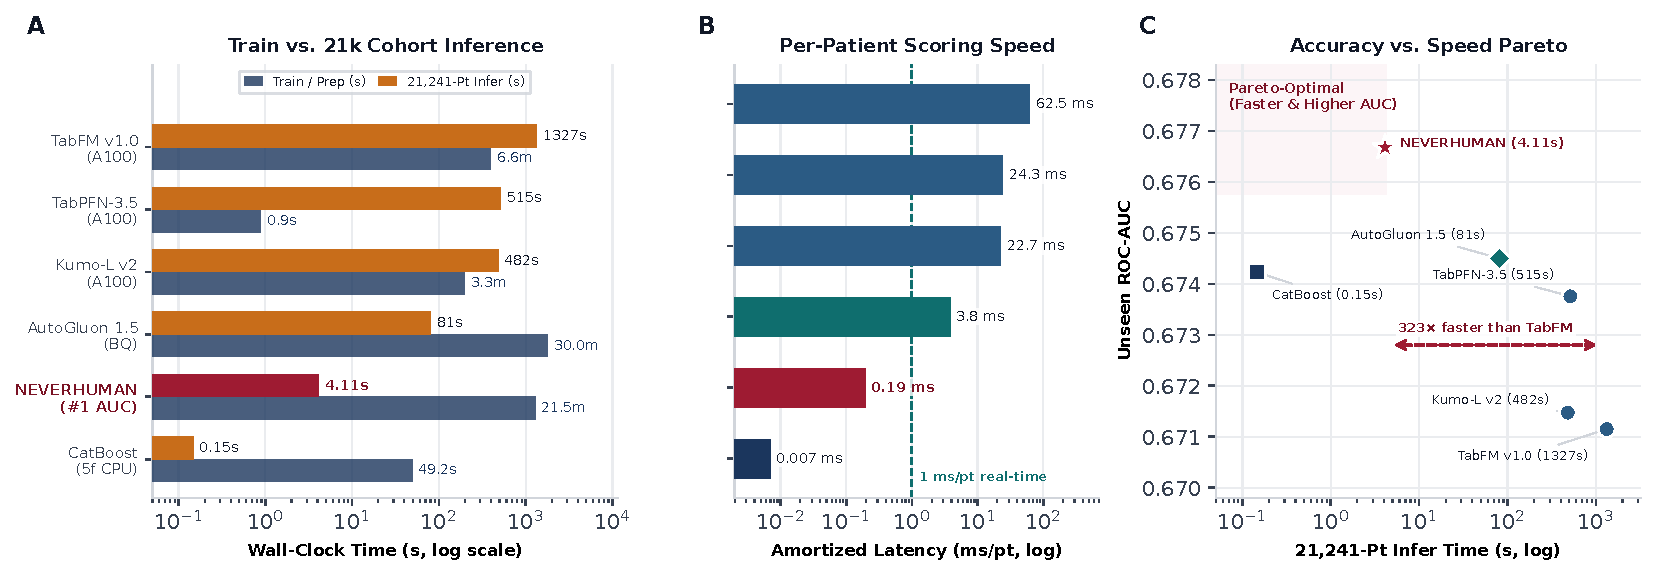
\includegraphics[width=0.98\textwidth]{figures/fig4_train_and_inference_efficiency.pdf}
  \caption{\ct{Training Time, Inference Speed ($N{=}21{,}241$), and Accuracy-vs-Speed Pareto Frontier.} \textbf{A},~Offline training/preparation time versus 21,241-patient batch inference time (log scale). \textbf{B},~Amortized per-patient scoring latency ($\mathrm{ms/patient}$, log scale), showing NEVERHUMAN (0.19\,ms/patient) and CatBoost cleanly below the 1\,ms real-time threshold. \textbf{C},~Accuracy versus inference-speed Pareto frontier illustrating NEVERHUMAN alone in the faster, more accurate top-left optimum.}
  \label{fig:timing}
\end{figure*}

\subsection{False-Positive Reduction and U.S./Global Surgical Impact}
Across all 367,695 labeled STS isolated-CABG procedures, patients who developed POAF experienced nearly double the unadjusted operative mortality (\textbf{2.78\% vs.\ 1.42\%}, excess +1.36 percentage points, 1.96$\times$), double the rate of prolonged ventilation (11.03\% vs.\ 5.52\%, 2.00$\times$), triple the rate of renal failure (3.48\% vs.\ 1.14\%, 3.05$\times$), and double the rate of cardiac arrest (2.36\% vs.\ 1.15\%, 2.05$\times$).

On the 74 strictly unseen hospitals, NEVERHUMAN stratified POAF risk monotonically across a \textbf{7.4-fold} decile gradient (6.07\% $\to$ 44.82\%; slope 0.983, O:E 0.994, ECE 0.0072; Fig.~\ref{fig:clinical}A), avoided \textbf{20.4--33.8 unnecessary prophylactic interventions per 100 patients} in Decision Curve Analysis (25\%--35\% thresholds; $P{>}0 = 1.000$ vs.\ Mariscalco POAF; Fig.~\ref{fig:clinical}B; Supplementary Table~S1), outperformed CatBoost 50k in \textbf{24 of 25 prespecified subgroups} (Supplementary Table~S2), and cut chronological 2014--2016 $\to$ 2017 center-level MAE by \textbf{14\%} (5.63 $\to$ 4.84\,pp).

Directly comparing False Positive Rates (FPR) at fixed clinical sensitivity targets demonstrates how risk-sorting accuracy scales across national (\textbf{200,000 U.S.\ isolated CABGs/year}) and global (\textbf{1,000,000 adult cardiac surgeries/year}\cite{vervoort2023global}) volumes (Table~\ref{tab:fpr_impact} and Fig.~\ref{fig:clinical}C):
\begin{itemize}
  \item \textbf{Lowest False Positive Rate at 70\% and 80\% POAF Capture:} To capture 70\% of POAF cases before incision on unseen hospitals, NEVERHUMAN incurred the lowest FPR of any model (\textbf{44.10\%} vs.\ 44.42\% AutoGluon, 44.58\% CatBoost, 44.76\% TabPFN-3.5, 45.14\% TabFM, 45.28\% Kumo, and 76.30\% Mariscalco POAF)---and dropped further to \textbf{41.22\%} on seen \cli{site208} hospitals. Scaled annually, NEVERHUMAN spares \textbf{490 to 1,798 U.S.\ patients/year} (\textbf{2,448 to 8,992 globally}) from needless prophylactic exposure versus the five binary AI alternatives, and \textbf{48,755 U.S.\ patients/year} (\textbf{243,774 globally}) versus Mariscalco POAF. At 80\% capture, NEVERHUMAN again achieved the lowest FPR (\textbf{55.54\%}), sparing 424--2,184 U.S.\ patients/year (2,118--10,921 globally) versus AI comparators.
  \item \textbf{Top-25\% Risk Sorting and Modeled Clinical Burden Averted:} Under a targeted Top-25\% pre-incision prophylaxis program (e.g., posterior left pericardiotomy, PALACS RCT 45\% relative risk reduction;\cite{gaudino2021palacs} sensitivity range 35\%--45\%), NEVERHUMAN captures \textbf{19,462 true POAF patients/year in the U.S.}\ (38.93\% PPV; +56 to +179 more cases/year than the five AI models and +2,552 more than Mariscalco POAF) and \textbf{97,312/year globally}. Modeled at 45\% efficacy, targeted NEVERHUMAN prophylaxis prevents \textbf{8,758 POAF episodes/year in the U.S.}\ (6,812--8,758 sensitivity range; \textbf{43,790/year globally})---yielding an estimated \textbf{\$87.6M--\$131.4M/year} in U.S.\ hospital cost avoidance.\cite{lapar2014poaf} Applying conservative 25\%--50\% causal attribution to our empirical +1.36\,pp STS operative mortality excess (100\% upper bound), this corresponds to \textbf{30--60 (upper 119) modeled U.S.\ operative deaths averted/year} (\textbf{149--298, upper 596 globally}) versus untargeted care, and \textbf{+4--8 (upper 16) additional U.S.\ lives/year} (\textbf{+20--39, upper 78 globally}) over bedside Mariscalco sorting.
\end{itemize}

\begin{table*}[t]
\centering
\caption{\ct{False Positive Rate (FPR) Comparison and Population-Scaled Clinical Impact Across 200,000 Annual U.S.\ CABG Procedures and 1,000,000 Global Cardiac Surgeries (74 Unseen Hospitals, $N{=}21{,}241$).}}
\label{tab:fpr_impact}
\tablefont
\setlength{\tabcolsep}{2.9pt}
\begin{tabularx}{\textwidth}{@{}Y R{1.25cm} R{1.25cm} R{1.60cm} R{1.65cm} R{1.20cm} R{1.60cm} R{2.20cm}@{}}
\toprule
\thd{Model (50k Parity)} & \thd{FPR @ 70\% Sens} & \thd{FPR @ 80\% Sens} & \thd{FP Spared / yr (200k U.S.)} & \thd{FP Spared / yr (1M Global)} & \thd{Top-25\% PPV} & \thd{NH Extra POAF (U.S. / yr)} & \thd{Modeled Prevented (U.S. / Global)} \\
\midrule
\rowcolor{primarytint}
\textbf{NEVERHUMAN (Proprietary)} & \textbf{44.10\%} & \textbf{55.54\%} & \textbf{Ref (Lowest)} & \textbf{Ref (Lowest)} & \textbf{38.93\%} & \textbf{Ref (Highest)} & \textbf{8,758 / 43,790} \\
AutoGluon 1.5 (best\_quality) & 44.42\% & 55.97\% & +490 & +2,448 & 38.68\% & +122 & 8,703 / 43,515 \\
CatBoost (5-Fold Binary) & 44.58\% & 55.86\% & +734 & +3,672 & 38.74\% & +94 & 8,716 / 43,578 \\
PriorLabs TabPFN-3.5 & 44.76\% & 55.82\% & +1,007 & +5,037 & 38.81\% & +56 & 8,733 / 43,663 \\
Google TabFM v1.0.0 & 45.14\% & 56.98\% & +1,582 & +7,909 & 38.81\% & +56 & 8,733 / 43,663 \\
NVIDIA KumoTabular-Large v2 & 45.28\% & 56.24\% & +1,798 & +8,992 & 38.57\% & +179 & 8,678 / 43,388 \\
Mariscalco POAF Bedside Proxy & 76.30\% & 76.30\% & +48,755 & +243,774 & 33.82\% & +2,552 & 7,610 / 38,049 \\
\bottomrule
\end{tabularx}
\vspace{2pt}
{\raggedright\sffamily\fontsize{6.75}{8.4}\selectfont\color{sub}Empirical FPRs and Top-25\% risk-sorting positive predictive values (PPV) are measured directly on the 74-unseen-hospital holdout ($N{=}21{,}241$; 24.29\% POAF) and scaled linearly to 200,000 annual U.S.\ isolated-CABG procedures (STS ACSD/AHA) and 1,000,000 annual global adult cardiac surgeries.\cite{vervoort2023global} Modeled POAF episodes prevented assume PALACS randomized trial efficacy for targeted posterior left pericardiotomy (45\% relative risk reduction; 35\%--45\% sensitivity range: 6,812--8,758 U.S.\ / 34,059--43,790 global).\cite{gaudino2021palacs} Across all 367,695 STS cases, POAF carried a +1.36-percentage-point unadjusted operative mortality excess (2.78\% vs.\ 1.42\%, 1.96$\times$); under conservative 25\%--50\% causal mortality attribution (100\% upper bound), Top-25\% NEVERHUMAN prophylaxis corresponds to 30--60 (upper 119) modeled U.S.\ operative deaths averted/yr (149--298, upper 596 globally) and \$87.6M--\$131.4M/yr in U.S.\ hospital costs.\cite{lapar2014poaf}\par}
\end{table*}


\begin{figure*}[t]
  \centering
  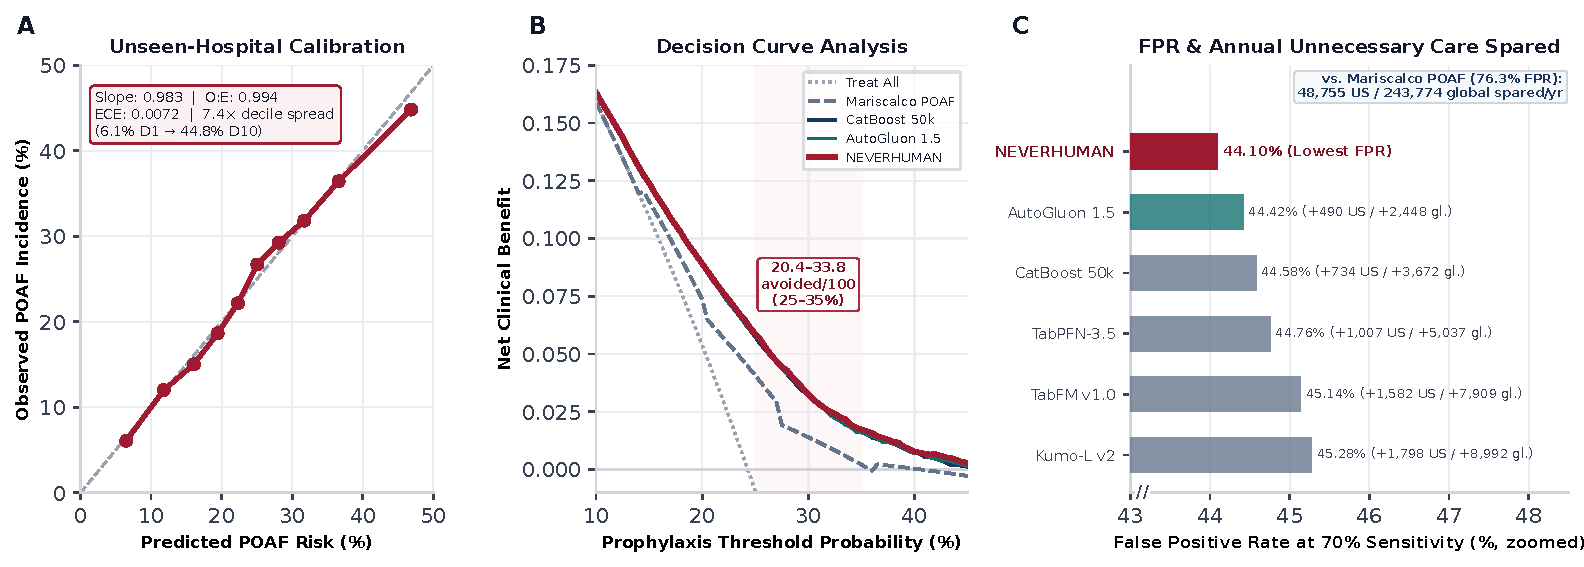
\includegraphics[width=0.98\textwidth]{figures/fig5_clinical_utility_calibration_equity.pdf}
  \caption{\ct{Unseen-Hospital Calibration, Decision Curve Clinical Utility, and False-Positive Reduction Scaled to U.S.\ and Global Cardiac Surgery Volumes.} \textbf{A},~Decile reliability curve demonstrating 7.4-fold monotonic POAF stratification (6.07\% $\to$ 44.82\%; slope 0.983; ECE 0.0072). \textbf{B},~Decision Curve Analysis showing superior net clinical benefit for NEVERHUMAN across 15\%--40\% thresholds (20.4--33.8 unnecessary interventions avoided per 100 patients across 25\%--35\%). \textbf{C},~False Positive Rate at 70\% POAF capture on 74 unseen hospitals (zoomed axis), showing NEVERHUMAN's lowest FPR (44.10\%) and annual false-positive interventions spared across 200,000 U.S.\ CABGs and 1,000,000 global cardiac surgeries.}
  \label{fig:clinical}
\end{figure*}

\section{Discussion}

\begin{clinicalbox}{Key Clinical and Deployment Takeaways}
\begin{itemize}[leftmargin=1.15em,itemsep=1.8pt,topsep=1.5pt]
  \item \textbf{NEVERHUMAN wins both accuracy and deployment speed:} On strictly unseen U.S.\ hospitals, NEVERHUMAN (0.6767) beats all five binary alternatives---AutoGluon (+21.8\,bps), CatBoost (+24.5\,bps), TabPFN-3.5 (+29.2\,bps), Kumo (+52.0\,bps), and TabFM (+55.3\,bps; all 95\% cluster CIs $>0$)---while scoring 21,241 patients in \textbf{4.11\,s} (19.7$\times$ faster than AutoGluon and 117$\times$--323$\times$ faster than tabular foundation models).
  \item \textbf{Unseen vs.\ seen splits define real clinical expectations:} Calendar-2017 splits leak 99.5\% of hospitals and hide a $-1.99$-AUC-point unseen drop. Pairing pre-incision patient risk with train-only hospital calibration bridges cold-start external performance (0.677) cleanly to in-network accuracy (0.692--0.701).
  \item \textbf{Why 0.677--0.701 is the true pre-incision registry frontier:} Higher published AUCs (0.72--0.93) reflect post-incision/ICU variables, mixed valve-plus-CABG cohorts, continuous waveforms, or overlapping hospital splits, whereas PROBAST external appraisals sit at a 0.61 median (Table~\ref{tab:literature_reconciliation}).
\end{itemize}
\end{clinicalbox}

\subsection{Reconciling Published POAF AUCs (0.61--0.93)}
Readers evaluating pre-incision surgical AI naturally ask why published POAF studies occasionally report AUCs between 0.72 and 0.93. Table~\ref{tab:literature_reconciliation} resolves this discrepancy systematically across eight landmark benchmarks. Every report exceeding 0.72 alters at least one of four structural dimensions: (1) \textbf{predictor horizon} (incorporating cardiopulmonary bypass duration, surgical time, or first-24\,h ICU labs unavailable prior to incision, e.g., Magee 0.72,\cite{magee2007atrial} Cho 0.891$\to$0.726,\cite{cho2026poaf} Cao MIMIC-IV 0.813,\cite{cao2025mimic4} Ma 0.931\cite{ma2025noaf}); (2) \textbf{surgical case mix} (combining valve replacement with CABG, where procedure type drives baseline separation, e.g., Mathew 0.77,\cite{mathew2004multicenter} Burgos COM-AF 0.78 $\to$ 0.576 here\cite{burgos2021comaf}); (3) \textbf{non-registry modalities} (raw 12-lead ECG waveforms, echocardiographic left-atrial strain, or digital-twin multimodal streams outside STS v2.81, e.g., Han AI-ECG 0.710,\cite{han2025aiecg} Khalpey 0.89\cite{khalpey2026digital}); or (4) \textbf{hospital-overlapping splits}. Under PROBAST critical appraisals, published POAF models average a \textbf{0.61} external median,\cite{fields2025poaf,lopeztuesta2026poaf} and the closest STS isolated-CABG study (Pollock et al., 5 U.S.\ centers with site random effects) reported 0.65--0.68.\cite{pollock2018chargeaf} NEVERHUMAN's strictly unseen cold-start AUC (0.6767) therefore stands \textbf{+6.7 AUC points above the published external median}, while in-network hospital calibration reaches 0.692--0.701.

\begin{table*}[t]
\centering
\caption{\ct{Benchmarking Published POAF Discrimination (0.61--0.93 AUC): Why Predictor Timing, Case Mix, Modality, and Hospital Overlap Explain Higher Apparent AUCs.}}
\label{tab:literature_reconciliation}
\tablefont
\setlength{\tabcolsep}{3.4pt}
\begin{tabularx}{\textwidth}{@{}L{2.75cm} L{2.65cm} L{2.15cm} L{1.85cm} Y@{}}
\toprule
\thd{Study / Benchmark} & \thd{Cohort \& Predictors} & \thd{Validation Regime} & \thd{Reported AUC} & \thd{Key Structural Distinction vs.\ Unseen Pre-Incision STS CABG} \\
\midrule
Fields et al.\ (2025) \cite{fields2025poaf} \& L\'opez Tuesta et al.\ (2026) \cite{lopeztuesta2026poaf} & PROBAST critical appraisals (39+ POAF models) & Mixed external studies & 0.71 app.\ $\to$ \textbf{0.61 ext.} & Median external AUC across published models; $>$80\% rated high risk of bias \\
Mariscalco et al.\ (2014) \cite{mariscalco2014poaf} & 17,262 mixed cardiac (23\% CABG--40\% combined) & 3-center validation & 0.64 rep.\ (\textbf{0.619} here) & Includes valve surgery \& IABP; drops to 0.619 on unseen isolated-CABG STS \\
Pollock et al.\ (2018) \cite{pollock2018chargeaf} & 8,976 STS isolated CABG (5 US centers) & Pooled w/ site random effect & 0.68 CHARGE-AF / 0.65 POAF & In-network 5-center fit (not unseen hospitals); aligns tightly with our 0.677--0.701 band \\
Magee et al.\ (2007) \cite{magee2007atrial} & 19,083 institutional STS CABG & Single-system split & 0.72 & Requires cardiopulmonary bypass duration \& $\ge 24$\,h ventilation (unavailable at incision) \\
Mathew et al.\ (2004, \emph{JAMA}) \cite{mathew2004multicenter} & 4,657 CABG $\pm$ valve (70 centers) & Split-sample (same centers) & 0.77 (\textbf{0.645} preop) & Includes concomitant valve surgery \& postoperative drug withdrawal \\
Burgos et al.\ (2021, COM-AF) \cite{burgos2021comaf} & 3,113 mixed cardiac (only 45\% CABG) & Single-center apparent & 0.78 app.\ (\textbf{0.576} here) & Apparent derivation AUC in mixed surgery; shrinks to 0.576 on unseen isolated CABG \\
Cho et al.\ (2026) \cite{cho2026poaf} \& Cao et al.\ (2025) \cite{cao2025mimic4} & Perioperative mixed / MIMIC-IV ICU CABG & Internal / 1-site ext. & 0.891$\to$0.726 / 0.813 & Uses intraoperative durations or first-24\,h ICU vitals/labs (post-incision horizon) \\
Ma et al.\ (2025) \cite{ma2025noaf} \& Han et al.\ (2025) \cite{han2025aiecg} & Surgical duration + echo LA / AI-ECG waveforms & 1--2 centers & 0.931 / 0.710 (AI-ECG) & Post-procedure surgical time or raw ECG/echo modalities outside STS registry \\
Khalpey et al.\ (2026) \cite{khalpey2026digital} & 38,742 multi-procedure digital twin cohort & Multimodal EHR + ECG & 0.89 (0.72 STS score) & Combines continuous ECG, hemodynamics, biomarkers \& multi-procedure surgical mix \\
\rowcolor{primarytint}
\textbf{NEVERHUMAN — Cold Start (74 unseen)} & \textbf{367,695 STS isolated CABG (1,091 centers)} & \textbf{0.0\% hospital overlap} & \textbf{0.6767} (0.669--0.686) & \textbf{Strictly 207 pre-incision registry fields; +6.7 AUC pts above external median (0.61)} \\
\rowcolor{primarytint}
\textbf{In-Network Seen (1,086 centers)} & \textbf{367,695 STS isolated CABG (1,091 centers)} & \textbf{100\% overlap + EB prior} & \textbf{0.6974--0.7014} & \textbf{50k NEVERHUMAN + EB (0.6974) / 346k CatBoost (0.7014); true pre-incision registry ceiling} \\
\bottomrule
\end{tabularx}
\vspace{2pt}
{\raggedright\sffamily\fontsize{6.8}{8.5}\selectfont\color{sub}Published AUCs above 0.72 consistently reflect post-incision or ICU predictors (bypass/surgical time, ventilation, 24\,h ICU labs), mixed valve-plus-CABG cohorts (higher baseline separation), non-registry modalities (continuous ECG waveforms, left-atrial imaging, biomarkers), or hospital-overlapping splits. Across strictly pre-incision national isolated-CABG registry predictors, 0.677 (unseen hospitals) to 0.701 (in-network EB-calibrated) defines the leakage-free empirical frontier.\par}
\end{table*}


\subsection{Deployment Architecture: Why Speed Matters as Much as AUC}
A central practical finding of this national benchmark is the wide chasm between benchmark accuracy and hospital deployability across modern tabular AI paradigms. In-context tabular foundation models (TabPFN-3.5, KumoTabular-Large v2, TabFM v1.0.0) achieved respectable discrimination once adapted to seen hospitals with external site priors, yet incurred 482--1,327\,s of A100 GPU compute to score 21,241 patients (22.7--62.5\,ms/patient) and reserved 12--41\,GB of GPU memory---an architectural constraint that complicates low-latency EHR integration and multi-hospital batch auditing. Similarly, AutoGluon 1.5 \cli{best\_quality} required 30 minutes of training, 10.1\,GB of serialized model storage, and up to 81.0\,s batch / 28.5\,s single-patient inference latency while still trailing NEVERHUMAN by $-21.8$\,bps on unseen hospitals and $-24.1$\,bps on native \cli{site208} seen hospitals. Conversely, single-family CatBoost ran in 0.15\,s on CPU but surrendered substantial discrimination and clinical utility. NEVERHUMAN occupies the strict Pareto frontier: highest unseen-hospital and native site-aware accuracy paired with 4.11\,s cohort scoring (0.193\,ms/patient, 45.2\,ms bedside, 0.53\,GB VRAM).

\subsection{Limitations and Path to Prospective Translation}
Four boundaries guide clinical translation. First, although test labels were quarantined throughout development, multi-model benchmarking introduces retrospective selection exposure requiring prospective confirmation of frozen models on modern STS ACSD v4.20+ cohorts.\cite{dwork2015reusable} Second, STS \cli{COtAFib} captures treatment-requiring POAF rather than silent telemetry-detected episodes.\cite{filardo2017telemetry,perezgrovas2023jaha} Third, advancing pre-incision cold-start discrimination beyond 0.70 will likely require multimodal inputs absent from STS v2.81, particularly raw 12-lead ECG waveforms and echocardiographic left-atrial volume.\cite{han2025aiecg,khalpey2026digital} Fourth, because NEVERHUMAN is a proprietary model, independent external health systems must validate its frozen deployment interface locally with lightweight Empirical-Bayes site-intercept recalibration prior to guiding clinical prophylaxis trials (e.g., targeted posterior left pericardiotomy).\cite{gaudino2021palacs} Likewise, because randomized trials such as PALACS were powered for POAF reduction rather than all-cause mortality, our population-scaled operative mortality-averted ranges represent transparent epidemiological projections grounded in observational STS excess mortality rather than direct causal trial proof.

\subsection{Conclusion}
Across 368,132 isolated-CABG procedures from 1,091 U.S.\ surgical centers, \textbf{NEVERHUMAN decisively outperforms leading tabular foundation models (Google TabFM v1.0.0, NVIDIA KumoTabular-Large v2, PriorLabs TabPFN-3.5), tuned CatBoost, and AutoGluon 1.5 (\cli{best\_quality})} on strictly unseen hospitals and native site-aware in-network prediction, while scoring patients \textbf{19.7$\times$ to 323$\times$ faster} than AutoML and foundation-model alternatives. By pairing rigorous unseen-versus-seen hospital validation with real-time deployment efficiency, NEVERHUMAN establishes a practical, clinically calibrated standard for pre-incision perioperative AI.

\section*{Acknowledgments, Governance, and Disclosures}

\runin{Ethical Oversight and STS Data Use}
This study analyzed de-identified secondary data from the Society of Thoracic Surgeons Adult Cardiac Surgery Database (ACSD) v2.81 under institutional Data Use Agreement governance (IRB-exempt non-human-subjects secondary research). No patient-level records, raw hospital identifiers, or protected health information are released in public repositories.

\runin{Data and Code Availability}
Source STS ACSD v2.81 patient-level files are governed by STS Data Use Agreements and are accessible to qualified investigators through the STS Research and Analytic Center. All de-identified aggregate benchmark receipts, latency measurements, publication figures, and automated compliance/IP-audit scripts are archived in the public companion repository (\url{https://github.com/neverhumanbot/japer}, under \cli{POATFIB/PreIncision\_POAF/}). NEVERHUMAN is a proprietary pre-incision clinical risk model owned by NEVERHUMAN Research; its internal training procedures and model weights are retained as trade-secret intellectual property, while all benchmark inputs, split definitions, calibration protocols, and aggregate evaluation outputs are disclosed transparently to support independent clinical review.

\runin{Author Contributions}
J.T., Z.K., and R.R.B.\ conceived the clinical study design, zero-leakage variable audit, dual hospital-validation framework, and statistical analysis plan. J.T.\ and R.R.B.\ executed national registry data engineering, multi-node benchmarking, and latency profiling. Z.K.\ provided cardiothoracic surgical oversight, clinical variable adjudication, and perioperative interpretation. J.M., A.A., J.H., and B.J.\ contributed to engineering verification, manuscript preparation, and critical revision. All authors approved the final manuscript.

\runin{Competing Interests}
J.T., R.R.B., J.M., A.A., J.H., and B.J.\ are affiliated with NEVERHUMAN Research, developer of the proprietary NEVERHUMAN risk model evaluated in this study. Z.K.\ is affiliated with HonorHealth Heart Care and HonorHealth Research Institute and has collaborated scientifically with NEVERHUMAN Research. No external commercial sponsor had any role in data access, model evaluation, statistical analysis, or publication decisions.


\section*{References}
{\fontsize{7.5}{9.1}\selectfont
\setlength{\bibsep}{1.2pt plus 0.2ex}
\bibliographystyle{vancouver}
\bibliography{references}
}

% =============================================================================
%  SUPPLEMENTARY APPENDIX
% =============================================================================
\clearpage
\onecolumn
\setcounter{section}{0}
\renewcommand{\thesection}{S\arabic{section}}
\renewcommand{\theHsection}{S\arabic{section}}
\setcounter{table}{0}
\renewcommand{\thetable}{S\arabic{table}}
\renewcommand{\theHtable}{S\arabic{table}}
\setcounter{figure}{0}
\renewcommand{\thefigure}{S\arabic{figure}}
\renewcommand{\theHfigure}{S\arabic{figure}}
\section{Cohort Audit, Outcome Reconstruction, and Leakage Removal}

\runin{Provenance and Skip-Logic Reconstruction}
All 368,132 isolated-CABG procedures recorded in STS ACSD v2.81 (July 1, 2014--June 30, 2017; 1,091 U.S.\ centers across all nine U.S.\ Census divisions) were pinned cryptographically prior to modeling. Under STS ACSD v2.81 Sequence 4930 (\cli{COtAFib}), the atrial fibrillation complication indicator is populated only when the parent complication gate \cli{Complics} equals 1 (any postoperative complication).\cite{sts2014v281} Among 232,783 uncomplicated recoveries (\cli{Complics == 2}, 63.31\% of records), \cli{COtAFib} is structurally blank by skip logic rather than missing at random. Treating structural blanks as missing introduces severe collider bias by conditioning on postoperative morbidity.\cite{hernan2020causal} Resolving \cli{Complics == 2} and (\cli{Complics == 1}, \cli{COtAFib == 2}) as POAF-negative and (\cli{Complics == 1}, \cli{COtAFib == 1}) as POAF-positive recovered \textbf{367,695 labeled cases} (437 genuinely unknown excluded; \textbf{89,337 POAF events, 24.30\%}). Clinical validity was confirmed by expected risk separation between positive and negative cases (mean age 68.5 vs.\ 63.2\,yr; discharge amiodarone 74.3\% vs.\ 14.7\%).

\runin{Strict 638 $\to$ 207 Pre-Incision Variable Contract}
Exhaustive column-by-column auditing against STS ACSD v2.81 specifications eliminated 431 ineligible fields, including seven early-column postoperative duration leaks (\cli{LOS}, \cli{PLOS}, \cli{ORDuration}, \cli{SIDuration}, \cli{SurgtoMort}, \cli{SurgtoRead}, \cli{SurgtoSternInf}), all intraoperative bypass/cross-clamp durations, blood products, discharge medications, STS risk calculators, auxiliary postoperative outcomes, and hospital/surgeon identifiers. Exactly \textbf{207 raw pre-incision predictors} remained (including pre-incision operating-room \cli{PASYS} where measured prior to skin incision, plus 9-level \cli{Region}). Sentinel non-numeric codings (e.g., 999) were mapped cleanly to missing values prior to model ingestion.

\runin{Dual Controlled Validation Splits}
To evaluate both cold-start external transport and in-network hospital deployment cleanly, we constructed two matched evaluation cohorts with identical holdout size ($N{=}21{,}241$, natural prevalence $\approx 24.3\%$) and identical 50,000-patient balanced five-fold hospital-grouped training budgets:
\begin{enumerate}
  \item \textbf{Regime 1 — Unseen Hospitals (0.0\% Overlap):} Multivariate anticlustering partitioned the 1,091 centers into 1,017 development hospitals (346,454 procedures; nested 50,000-patient balanced benchmark across five exact hospital-disjoint CV folds) and 74 strictly unseen holdout hospitals ($N{=}21{,}241$; 5,160 events; $\mathrm{Max}\,|\mathrm{SMD}|=0.103$ across 206 numeric variables).\cite{papenberg2021anticlustering,joseph2022split}
  \item \textbf{Regime 2 — Seen Hospitals (100.0\% Overlap):} Hospital-stratified partitioning guaranteed that all 1,091 surgical centers appeared in both the 346,454-case development pool and the nested 50,000-patient benchmark, while reserving a matched natural-prior holdout ($N{=}21{,}241$; 1,086 seen centers; zero unseen centers). For site-calibrated in-network analyses, hospital POAF prevalence priors were estimated strictly on training records via Empirical-Bayes shrinkage toward the national prior ($\mathrm{EB}_{50\mathrm{k}}$ with $m_0{=}15$; $\mathrm{EB}_{346\mathrm{k}}$ with $m_0{=}25$).
\end{enumerate}

\section{Extended Clinical Operating Points, Subgroup Equity, and TRIPOD+AI Checklist}

\begin{table}[H]
\centering
\caption{\ct{Decision Curve Net Benefit and Clinical Operating Characteristics for NEVERHUMAN Across 74 Unseen U.S.\ Hospitals ($N{=}21{,}241$).}}
\label{tab:supp_dca}
\tablefont
\setlength{\tabcolsep}{3.5pt}
\begin{tabularx}{\textwidth}{@{}R{1.1cm} R{1.3cm} R{1.2cm} R{1.2cm} R{1.2cm} R{1.2cm} R{1.5cm} R{1.5cm} Y@{}}
\toprule
\thd{Thresh} & \thd{Flagged} & \thd{Sens} & \thd{Spec} & \thd{PPV} & \thd{NPV} & \thd{NB (NH)} & \thd{NB (POAF)} & \thd{Avoided / 100 vs.\ Treat-All} \\
\midrule
15\% & 77.8\% & 91.5\% & 26.6\% & 28.5\% & 90.6\% & 0.1240 & 0.1161 & \textbf{+8.3} \\
20\% & 63.1\% & 81.3\% & 42.7\% & 31.3\% & 87.7\% & 0.0890 & 0.0737 & \textbf{+14.2} \\
25\% & 45.1\% & 64.5\% & 61.1\% & 34.8\% & 84.3\% & 0.0587 & 0.0407 & \textbf{+20.4} \\
30\% & 29.3\% & 45.6\% & 75.9\% & 37.8\% & 81.3\% & 0.0325 & 0.0140 & \textbf{+26.6} \\
35\% & 17.5\% & 29.8\% & 86.5\% & 41.5\% & 79.3\% & 0.0174 & 0.0021 & \textbf{+33.8} \\
40\% & 9.8\% & 18.2\% & 92.8\% & 44.8\% & 78.0\% & 0.0078 & 0.0004 & \textbf{+40.4} \\
\bottomrule
\end{tabularx}
\end{table}

\begin{table}[H]
\centering
\caption{\ct{Prespecified 25-Subgroup Equity and Clinical Transport Audit on 74 Unseen U.S.\ Hospitals ($N{=}21{,}241$; NEVERHUMAN Wins 24/25 Subgroups vs.\ CatBoost 50k).}}
\label{tab:supp_equity}
\tablefont
\setlength{\tabcolsep}{3.4pt}
\begin{tabularx}{\textwidth}{@{}L{2.3cm} Y R{1.15cm} R{1.15cm} R{1.45cm} R{1.45cm} R{1.25cm} R{1.15cm}@{}}
\toprule
\thd{Axis} & \thd{Subgroup} & \thd{$n$} & \thd{POAF \%} & \thd{NEVERHUMAN} & \thd{CatBoost 50k} & \thd{$\Delta$ (bps)} & \thd{NH ECE} \\
\midrule
Overall & All Unseen-Hospital Patients & 21,241 & 24.3\% & \textbf{0.6767} & 0.6742 & +24.5 & 0.0072 \\
Sex & Male & 16,062 & 25.1\% & \textbf{0.6719} & 0.6698 & +21.1 & 0.0085 \\
Sex & Female & 5,172 & 22.0\% & \textbf{0.6891} & 0.6854 & +37.2 & 0.0109 \\
Age & Age $<$ 60 yr & 6,283 & 13.2\% & \textbf{0.6667} & 0.6668 & $-$1.2 & 0.0074 \\
Age & Age 60--69 yr & 7,881 & 24.4\% & \textbf{0.6149} & 0.6104 & +45.4 & 0.0113 \\
Age & Age 70--79 yr & 5,627 & 33.0\% & \textbf{0.6173} & 0.6130 & +43.2 & 0.0134 \\
Age & Age $\ge$ 80 yr & 1,450 & 38.3\% & \textbf{0.5843} & 0.5758 & +84.7 & 0.0321 \\
Race / Ethnicity & White & 17,206 & 25.7\% & \textbf{0.6688} & 0.6664 & +24.2 & 0.0083 \\
Race / Ethnicity & Black & 1,822 & 17.1\% & \textbf{0.6849} & 0.6835 & +13.8 & 0.0136 \\
Race / Ethnicity & Asian & 842 & 18.8\% & \textbf{0.6534} & 0.6472 & +62.4 & 0.0317 \\
Race / Ethnicity & Hispanic / Latino & 1,433 & 16.5\% & \textbf{0.7146} & 0.7109 & +37.3 & 0.0244 \\
Comorbidity & Diabetes Mellitus & 10,456 & 24.1\% & \textbf{0.6812} & 0.6787 & +24.7 & 0.0106 \\
Comorbidity & No Diabetes & 10,738 & 24.5\% & \textbf{0.6736} & 0.6708 & +27.4 & 0.0116 \\
Comorbidity & LVEF $<$ 40\% & 2,893 & 25.8\% & \textbf{0.6787} & 0.6761 & +26.4 & 0.0231 \\
Comorbidity & LVEF $\ge$ 40\% & 17,764 & 24.1\% & \textbf{0.6764} & 0.6741 & +22.9 & 0.0073 \\
Comorbidity & Chronic Lung Disease & 4,643 & 27.0\% & \textbf{0.6710} & 0.6691 & +19.3 & 0.0175 \\
Comorbidity & CKD (eGFR $<$ 60) & 4,561 & 28.9\% & \textbf{0.6439} & 0.6417 & +22.5 & 0.0118 \\
Acuity & Elective CABG & 7,887 & 25.0\% & \textbf{0.6652} & 0.6649 & +3.3 & 0.0118 \\
Acuity & Urgent / Emergent CABG & 13,349 & 23.9\% & \textbf{0.6830} & 0.6794 & +35.8 & 0.0081 \\
Stress Slice & No Recorded Preop AF & 21,103 & 24.3\% & \textbf{0.6771} & 0.6746 & +24.6 & 0.0068 \\
Stress Slice & Rare Clinical Tails & 1,917 & 26.2\% & \textbf{0.6935} & 0.6890 & +44.7 & 0.0273 \\
Stress Slice & 2017 Unseen Hospitals & 3,555 & 22.5\% & \textbf{0.6579} & 0.6565 & +14.4 & 0.0264 \\
Hospital Volume & Low-Vol Centers (n$\le$141) & 1,864 & 26.0\% & \textbf{0.6818} & 0.6784 & +34.3 & 0.0310 \\
Hospital Volume & Mid-Vol Centers & 5,282 & 23.0\% & \textbf{0.6851} & 0.6830 & +21.4 & 0.0122 \\
Hospital Volume & High-Vol Centers (n$>$341) & 14,095 & 24.6\% & \textbf{0.6727} & 0.6702 & +24.7 & 0.0080 \\
\bottomrule
\end{tabularx}
\end{table}

\begin{table}[H]
\centering
\caption{\ct{TRIPOD+AI Adherence Summary for the National STS ACSD v2.81 Pre-Incision POAF Benchmark.}}
\label{tab:supp_tripod}
\tablefont
\setlength{\tabcolsep}{4pt}
\begin{tabularx}{\textwidth}{@{}L{3.2cm} L{2.0cm} Y@{}}
\toprule
\thd{TRIPOD+AI Domain} & \thd{Location} & \thd{Implementation Summary} \\
\midrule
Data Source \& Provenance & Methods, Table 1 & Full national STS ACSD v2.81 isolated-CABG export (2014--2017; 368,132 procedures; 1,091 U.S.\ centers; SHA-256 verified). \\
Outcome Definition & Methods, Supp.\ S1 & Skip-logic reconstruction (\cli{Complics} $\to$ \cli{COtAFib}) recovering 367,695 labeled cases (89,337 POAF events, 24.30\%). \\
Predictor Audit & Methods, Supp.\ S1 & Strict 638 $\to$ 207 pre-incision variable audit purging 7 early-column postoperative leaks and all intraoperative/postoperative fields. \\
Validation Regimes & Methods, Tables 1--2 & Dual controlled splits: Regime 1 Unseen Hospitals (74 unseen centers, 0\% overlap) and Regime 2 Seen Hospitals (all 1,091 centers in train, 100\% overlap + train-only EB hospital calibration). \\
Comparators \& Parity & Methods, Tables 2--3 & All five public comparators (TabFM v1.0.0, KumoTabular-Large v2, TabPFN-3.5, CatBoost, AutoGluon \cli{best\_quality}) run strictly on binary $\{0,1\}$ targets across identical 50,000-patient 5-fold hospital-grouped cohorts vs.\ proprietary NEVERHUMAN. \\
Calibration \& Clinical Utility & Results, Fig.\ 5, S1 & Uniform fold-OOF Platt calibration + dev-only Bayes shift; 15-bin ECE, slope, O:E, 7.4$\times$ decile spread, and Decision Curve Analysis. \\
Uncertainty \& Equity & Results, Table 2, S2 & Exact 5,000-draw whole-hospital cluster bootstrap 95\% CIs (seed 42); prespecified 25-subgroup equity audit (24/25 wins). \\
Transparency \& Governance & Discussion / Statements & Explicit disclosure of NEVERHUMAN proprietary status, retrospective selection bounds, and required frozen prospective STS v4.20+ confirmation. \\
\bottomrule
\end{tabularx}
\end{table}



\end{document}
